\documentclass{standalone}
\usepackage{tikz}
\usetikzlibrary{patterns, positioning}
\usepackage[sfdefault]{ClearSans} %% option 'sfdefault' activates Clear Sans as the default text font
\usepackage[T1]{fontenc}

\begin{document}
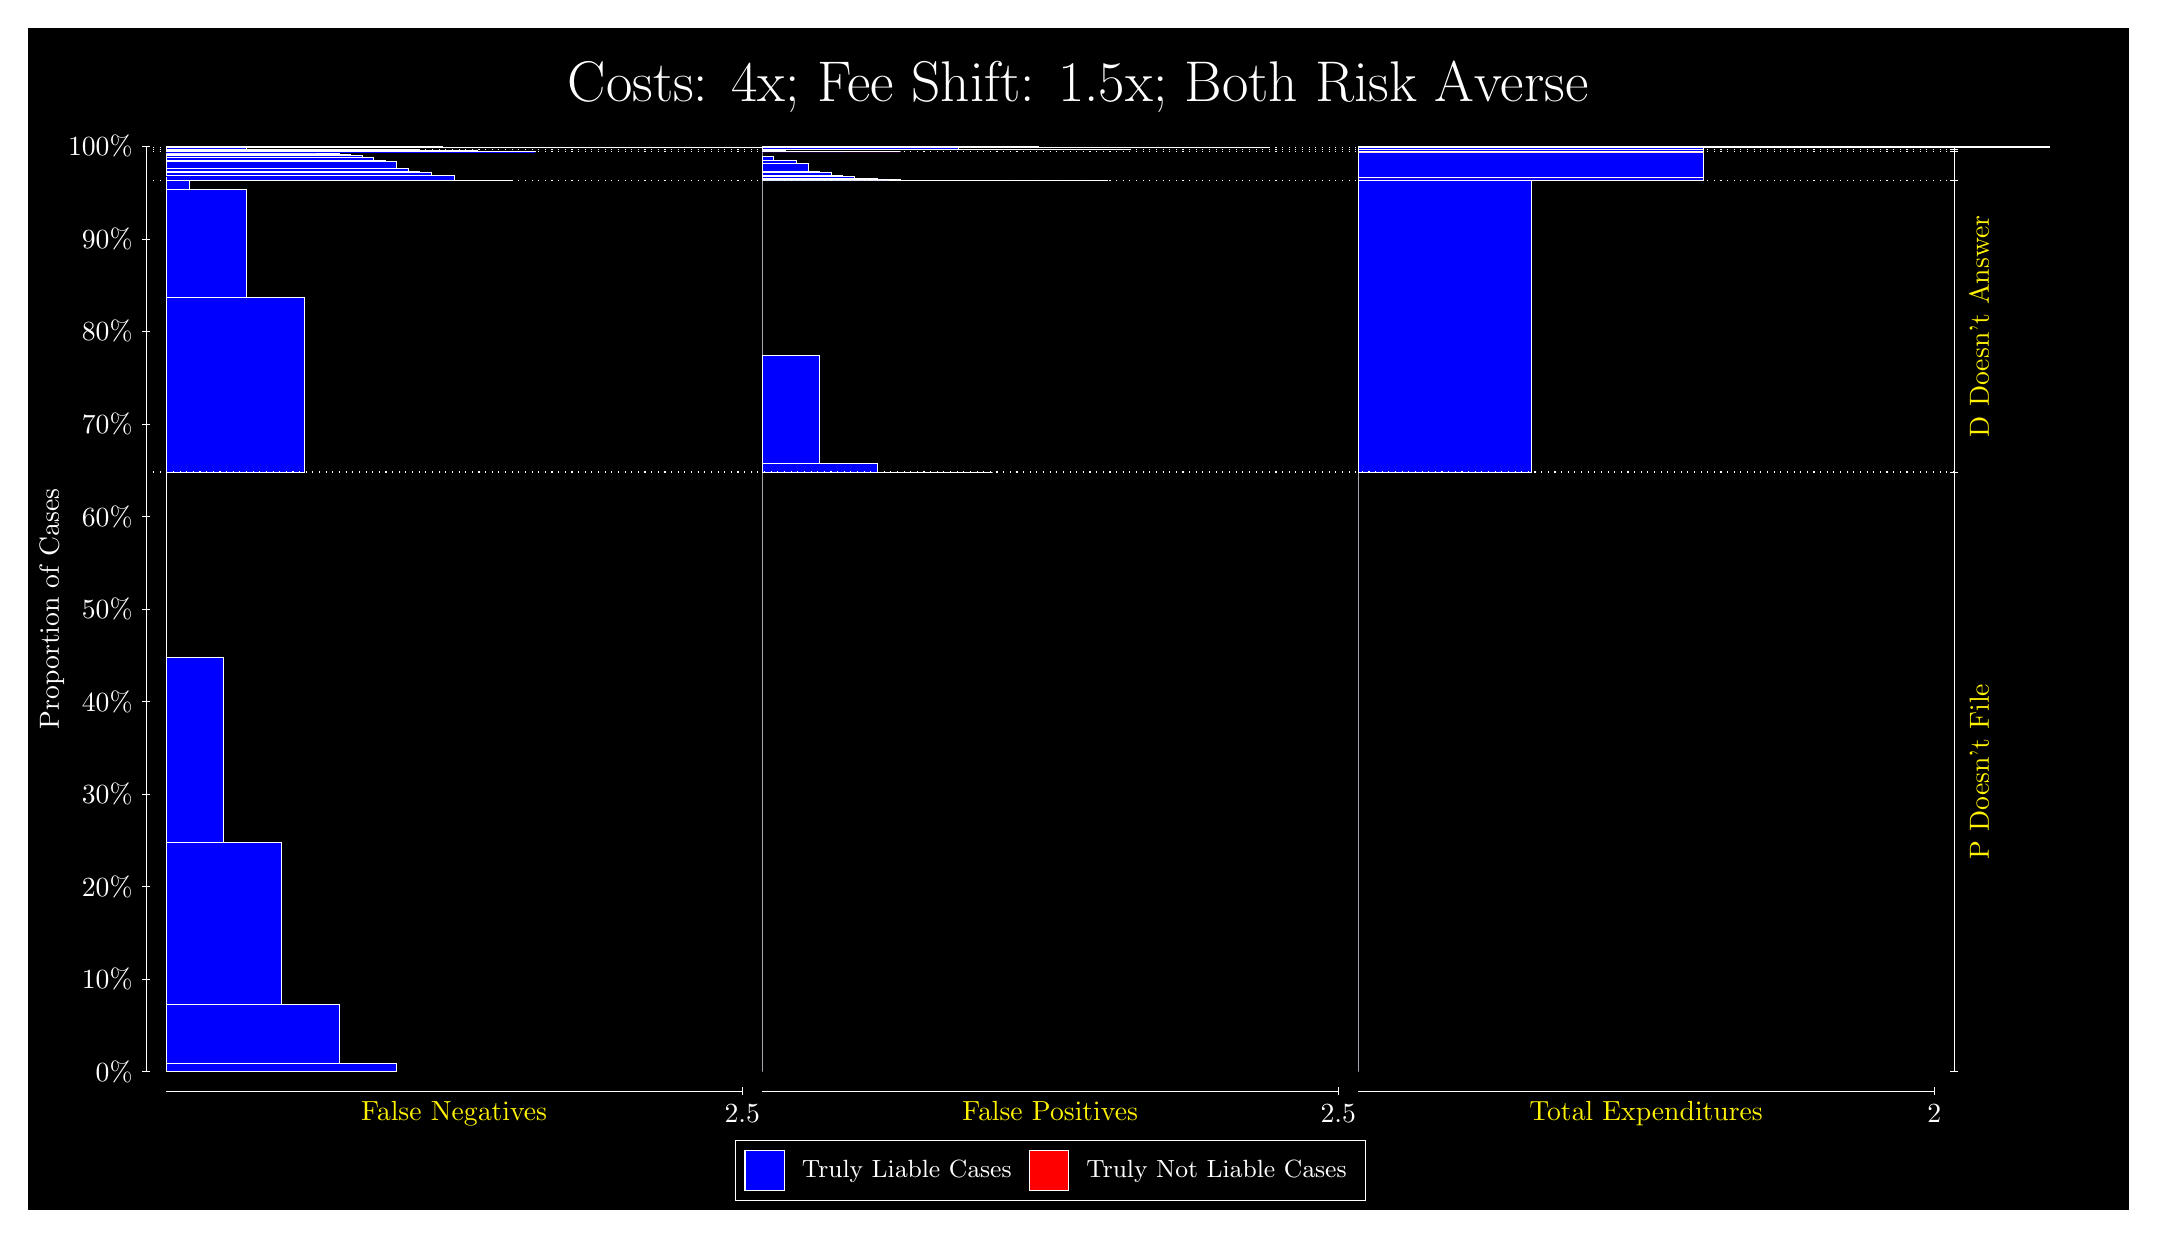
\begin{tikzpicture}
\draw[fill=black] (0,0) rectangle (26.667,15);
\draw[text=white] (0,13.5) rectangle (26.667,15) node[midway] {\huge Costs: 4x; Fee Shift: 1.5x; Both Risk Averse};
\draw[white, very thin] (1.5,1.75) -- (1.5,13.5);
\node[rotate=90, text=white, anchor=center] at (0.3, 7.625) {Proportion of Cases};
\draw[white, very thin] (1.45,1.75) -- (1.55,1.75);
\node[text=white, anchor=east] at (1.45, 1.75) {0\%};
\draw[white, very thin] (1.45,2.925) -- (1.55,2.925);
\node[text=white, anchor=east] at (1.45, 2.925) {10\%};
\draw[white, very thin] (1.45,4.1) -- (1.55,4.1);
\node[text=white, anchor=east] at (1.45, 4.1) {20\%};
\draw[white, very thin] (1.45,5.275) -- (1.55,5.275);
\node[text=white, anchor=east] at (1.45, 5.275) {30\%};
\draw[white, very thin] (1.45,6.45) -- (1.55,6.45);
\node[text=white, anchor=east] at (1.45, 6.45) {40\%};
\draw[white, very thin] (1.45,7.625) -- (1.55,7.625);
\node[text=white, anchor=east] at (1.45, 7.625) {50\%};
\draw[white, very thin] (1.45,8.8) -- (1.55,8.8);
\node[text=white, anchor=east] at (1.45, 8.8) {60\%};
\draw[white, very thin] (1.45,9.975) -- (1.55,9.975);
\node[text=white, anchor=east] at (1.45, 9.975) {70\%};
\draw[white, very thin] (1.45,11.15) -- (1.55,11.15);
\node[text=white, anchor=east] at (1.45, 11.15) {80\%};
\draw[white, very thin] (1.45,12.325) -- (1.55,12.325);
\node[text=white, anchor=east] at (1.45, 12.325) {90\%};
\draw[white, very thin] (1.45,13.5) -- (1.55,13.5);
\node[text=white, anchor=east] at (1.45, 13.5) {100\%};

\draw[white, very thin] (24.457,1.75) -- (24.457,13.5);
\draw[white, very thin] (24.407,1.75) -- (24.507,1.75);
\node[anchor=west] at (24.407, 1.75) {};
\draw[white, very thin] (24.407,9.3644) -- (24.507,9.3644);
\node[anchor=west] at (24.407, 9.3644) {};
\draw[white, very thin] (24.407,13.066) -- (24.507,13.066);
\node[anchor=west] at (24.407, 13.066) {};
\draw[white, very thin] (24.407,13.431) -- (24.507,13.431);
\node[anchor=west] at (24.407, 13.431) {};
\draw[white, very thin] (24.407,13.463) -- (24.507,13.463);
\node[anchor=west] at (24.407, 13.463) {};
\draw[white, very thin] (24.407,13.49) -- (24.507,13.49);
\node[anchor=west] at (24.407, 13.49) {};
\draw[white, very thin] (24.407,13.5) -- (24.507,13.5);
\node[anchor=west] at (24.407, 13.5) {};

\draw[white, very thin, fill=blue] (1.75,1.75) rectangle (4.6775,1.8561);
\draw[white, very thin, fill=blue] (1.75,1.8561) rectangle (3.9457,2.6036);
\draw[white, very thin, fill=blue] (1.75,2.6036) rectangle (3.2138,4.6668);
\draw[white, very thin, fill=blue] (1.75,4.6668) rectangle (2.4819,7.0144);
\draw[white, very thin, fill=red] (1.75,7.0144) rectangle (1.75,7.0144);
\draw[white, very thin, fill=blue] (1.75,7.0144) rectangle (1.75,9.3644);
\draw[white, very thin, fill=blue] (1.75,9.3644) rectangle (3.5065,11.584);
\draw[white, very thin, fill=blue] (1.75,11.584) rectangle (2.7746,12.958);
\draw[white, very thin, fill=blue] (1.75,12.958) rectangle (2.0428,13.066);
\draw[white, very thin, fill=red] (1.75,13.066) rectangle (1.75,13.066);
\draw[white, very thin, fill=blue] (1.75,13.066) rectangle (1.75,13.066);
\draw[white, very thin, fill=blue] (1.75,13.066) rectangle (6.1413,13.067);
\draw[white, very thin, fill=blue] (1.75,13.067) rectangle (5.8486,13.068);
\draw[white, very thin, fill=blue] (1.75,13.068) rectangle (5.5558,13.071);
\draw[white, very thin, fill=blue] (1.75,13.071) rectangle (5.4094,13.127);
\draw[white, very thin, fill=blue] (1.75,13.127) rectangle (5.2631,13.129);
\draw[white, very thin, fill=blue] (1.75,13.129) rectangle (5.1167,13.174);
\draw[white, very thin, fill=blue] (1.75,13.174) rectangle (4.9703,13.179);
\draw[white, very thin, fill=blue] (1.75,13.179) rectangle (4.8239,13.219);
\draw[white, very thin, fill=blue] (1.75,13.219) rectangle (4.6775,13.31);
\draw[white, very thin, fill=blue] (1.75,13.31) rectangle (4.5312,13.324);
\draw[white, very thin, fill=blue] (1.75,13.324) rectangle (4.3848,13.326);
\draw[white, very thin, fill=blue] (1.75,13.326) rectangle (4.3848,13.361);
\draw[white, very thin, fill=blue] (1.75,13.361) rectangle (4.2384,13.383);
\draw[white, very thin, fill=blue] (1.75,13.383) rectangle (4.092,13.403);
\draw[white, very thin, fill=blue] (1.75,13.403) rectangle (4.092,13.403);
\draw[white, very thin, fill=blue] (1.75,13.403) rectangle (3.9457,13.409);
\draw[white, very thin, fill=blue] (1.75,13.409) rectangle (3.7993,13.416);
\draw[white, very thin, fill=blue] (1.75,13.416) rectangle (3.6529,13.42);
\draw[white, very thin, fill=blue] (1.75,13.42) rectangle (3.6529,13.42);
\draw[white, very thin, fill=blue] (1.75,13.42) rectangle (3.5065,13.429);
\draw[white, very thin, fill=blue] (1.75,13.429) rectangle (3.3602,13.429);
\draw[white, very thin, fill=blue] (1.75,13.429) rectangle (3.3602,13.429);
\draw[white, very thin, fill=blue] (1.75,13.429) rectangle (3.2138,13.43);
\draw[white, very thin, fill=blue] (1.75,13.43) rectangle (3.0674,13.43);
\draw[white, very thin, fill=blue] (1.75,13.43) rectangle (3.0674,13.43);
\draw[white, very thin, fill=blue] (1.75,13.43) rectangle (2.921,13.431);
\draw[white, very thin, fill=blue] (1.75,13.431) rectangle (2.921,13.431);
\draw[white, very thin, fill=blue] (1.75,13.431) rectangle (2.7746,13.431);
\draw[white, very thin, fill=blue] (1.75,13.431) rectangle (2.6283,13.431);
\draw[white, very thin, fill=blue] (1.75,13.431) rectangle (2.6283,13.431);
\draw[white, very thin, fill=blue] (1.75,13.431) rectangle (2.4819,13.431);
\draw[white, very thin, fill=blue] (1.75,13.431) rectangle (2.3355,13.431);
\draw[white, very thin, fill=blue] (1.75,13.431) rectangle (2.3355,13.431);
\draw[white, very thin, fill=blue] (1.75,13.431) rectangle (2.1891,13.431);
\draw[white, very thin, fill=blue] (1.75,13.431) rectangle (2.0428,13.431);
\draw[white, very thin, fill=blue] (1.75,13.431) rectangle (1.8964,13.431);
\draw[white, very thin, fill=red] (1.75,13.431) rectangle (1.75,13.431);
\draw[white, very thin, fill=blue] (1.75,13.431) rectangle (1.75,13.431);
\draw[white, very thin, fill=blue] (1.75,13.431) rectangle (6.4341,13.433);
\draw[white, very thin, fill=blue] (1.75,13.433) rectangle (5.7022,13.45);
\draw[white, very thin, fill=blue] (1.75,13.45) rectangle (4.9703,13.463);
\draw[white, very thin, fill=blue] (1.75,13.463) rectangle (4.2384,13.463);
\draw[white, very thin, fill=blue] (1.75,13.463) rectangle (3.5065,13.463);
\draw[white, very thin, fill=red] (1.75,13.463) rectangle (1.75,13.463);
\draw[white, very thin, fill=blue] (1.75,13.463) rectangle (3.5065,13.468);
\draw[white, very thin, fill=blue] (1.75,13.468) rectangle (2.7746,13.486);
\draw[white, very thin, fill=blue] (1.75,13.486) rectangle (2.0428,13.489);
\draw[white, very thin, fill=red] (1.75,13.489) rectangle (1.75,13.489);
\draw[white, very thin, fill=blue] (1.75,13.489) rectangle (1.75,13.49);
\draw[white, very thin, fill=blue] (1.75,13.49) rectangle (13.46,13.49);
\draw[white, very thin, fill=blue] (1.75,13.49) rectangle (12.728,13.49);
\draw[white, very thin, fill=blue] (1.75,13.49) rectangle (11.996,13.49);
\draw[white, very thin, fill=blue] (1.75,13.49) rectangle (11.265,13.49);
\draw[white, very thin, fill=blue] (1.75,13.49) rectangle (10.533,13.49);
\draw[white, very thin, fill=blue] (1.75,13.49) rectangle (9.8008,13.49);
\draw[white, very thin, fill=blue] (1.75,13.49) rectangle (9.0689,13.49);
\draw[white, very thin, fill=blue] (1.75,13.49) rectangle (7.4587,13.49);
\draw[white, very thin, fill=blue] (1.75,13.49) rectangle (6.7268,13.49);
\draw[white, very thin, fill=blue] (1.75,13.49) rectangle (5.9949,13.492);
\draw[white, very thin, fill=blue] (1.75,13.492) rectangle (5.2631,13.498);
\draw[white, very thin, fill=blue] (1.75,13.498) rectangle (4.5312,13.5);
\draw[white, very thin, fill=blue] (1.75,13.5) rectangle (3.7993,13.5);
\draw[white, very thin, fill=blue] (1.75,13.5) rectangle (3.0674,13.5);
\draw[white, very thin, fill=blue] (1.75,13.5) rectangle (2.3355,13.5);
\draw[white, very thin, fill=red] (1.75,13.5) rectangle (1.75,13.5);
\draw[white, very thin, fill=red] (9.3189,1.75) rectangle (9.3189,1.75);
\draw[white, very thin, fill=blue] (9.3189,1.75) rectangle (9.3189,9.3644);
\draw[white, very thin, fill=red] (9.3189,9.3644) rectangle (12.246,9.3644);
\draw[white, very thin, fill=blue] (9.3189,9.3644) rectangle (12.246,9.3644);
\draw[white, very thin, fill=blue] (9.3189,9.3644) rectangle (11.515,9.3645);
\draw[white, very thin, fill=blue] (9.3189,9.3645) rectangle (10.783,9.4724);
\draw[white, very thin, fill=blue] (9.3189,9.4724) rectangle (10.051,10.847);
\draw[white, very thin, fill=blue] (9.3189,10.847) rectangle (9.3189,13.066);
\draw[white, very thin, fill=red] (9.3189,13.066) rectangle (13.71,13.066);
\draw[white, very thin, fill=blue] (9.3189,13.066) rectangle (13.71,13.066);
\draw[white, very thin, fill=red] (9.3189,13.066) rectangle (13.417,13.066);
\draw[white, very thin, fill=blue] (9.3189,13.066) rectangle (13.417,13.066);
\draw[white, very thin, fill=red] (9.3189,13.066) rectangle (13.125,13.066);
\draw[white, very thin, fill=blue] (9.3189,13.066) rectangle (13.125,13.066);
\draw[white, very thin, fill=blue] (9.3189,13.066) rectangle (12.978,13.066);
\draw[white, very thin, fill=red] (9.3189,13.066) rectangle (12.832,13.066);
\draw[white, very thin, fill=blue] (9.3189,13.066) rectangle (12.832,13.066);
\draw[white, very thin, fill=blue] (9.3189,13.066) rectangle (12.686,13.066);
\draw[white, very thin, fill=red] (9.3189,13.066) rectangle (12.539,13.066);
\draw[white, very thin, fill=blue] (9.3189,13.066) rectangle (12.539,13.066);
\draw[white, very thin, fill=blue] (9.3189,13.066) rectangle (12.393,13.066);
\draw[white, very thin, fill=red] (9.3189,13.066) rectangle (12.246,13.066);
\draw[white, very thin, fill=blue] (9.3189,13.066) rectangle (12.246,13.066);
\draw[white, very thin, fill=blue] (9.3189,13.066) rectangle (12.1,13.066);
\draw[white, very thin, fill=red] (9.3189,13.066) rectangle (11.954,13.066);
\draw[white, very thin, fill=blue] (9.3189,13.066) rectangle (11.954,13.066);
\draw[white, very thin, fill=blue] (9.3189,13.066) rectangle (11.807,13.066);
\draw[white, very thin, fill=red] (9.3189,13.066) rectangle (11.661,13.066);
\draw[white, very thin, fill=blue] (9.3189,13.066) rectangle (11.661,13.066);
\draw[white, very thin, fill=blue] (9.3189,13.066) rectangle (11.661,13.067);
\draw[white, very thin, fill=blue] (9.3189,13.067) rectangle (11.515,13.067);
\draw[white, very thin, fill=red] (9.3189,13.067) rectangle (11.368,13.067);
\draw[white, very thin, fill=blue] (9.3189,13.067) rectangle (11.368,13.068);
\draw[white, very thin, fill=blue] (9.3189,13.068) rectangle (11.222,13.069);
\draw[white, very thin, fill=blue] (9.3189,13.069) rectangle (11.075,13.077);
\draw[white, very thin, fill=blue] (9.3189,13.077) rectangle (10.929,13.077);
\draw[white, very thin, fill=blue] (9.3189,13.077) rectangle (10.929,13.081);
\draw[white, very thin, fill=blue] (9.3189,13.081) rectangle (10.783,13.088);
\draw[white, very thin, fill=blue] (9.3189,13.088) rectangle (10.636,13.094);
\draw[white, very thin, fill=blue] (9.3189,13.094) rectangle (10.49,13.115);
\draw[white, very thin, fill=blue] (9.3189,13.115) rectangle (10.344,13.137);
\draw[white, very thin, fill=blue] (9.3189,13.137) rectangle (10.197,13.172);
\draw[white, very thin, fill=blue] (9.3189,13.172) rectangle (10.197,13.173);
\draw[white, very thin, fill=blue] (9.3189,13.173) rectangle (10.051,13.188);
\draw[white, very thin, fill=blue] (9.3189,13.188) rectangle (9.9044,13.279);
\draw[white, very thin, fill=blue] (9.3189,13.279) rectangle (9.758,13.318);
\draw[white, very thin, fill=blue] (9.3189,13.318) rectangle (9.6116,13.324);
\draw[white, very thin, fill=blue] (9.3189,13.324) rectangle (9.4652,13.369);
\draw[white, very thin, fill=blue] (9.3189,13.369) rectangle (9.3189,13.431);
\draw[white, very thin, fill=red] (9.3189,13.431) rectangle (11.075,13.431);
\draw[white, very thin, fill=blue] (9.3189,13.431) rectangle (11.075,13.431);
\draw[white, very thin, fill=blue] (9.3189,13.431) rectangle (10.344,13.431);
\draw[white, very thin, fill=blue] (9.3189,13.431) rectangle (9.6116,13.444);
\draw[white, very thin, fill=blue] (9.3189,13.444) rectangle (9.3189,13.463);
\draw[white, very thin, fill=red] (9.3189,13.463) rectangle (14.003,13.463);
\draw[white, very thin, fill=blue] (9.3189,13.463) rectangle (14.003,13.463);
\draw[white, very thin, fill=blue] (9.3189,13.463) rectangle (13.271,13.463);
\draw[white, very thin, fill=blue] (9.3189,13.463) rectangle (12.539,13.466);
\draw[white, very thin, fill=blue] (9.3189,13.466) rectangle (11.807,13.485);
\draw[white, very thin, fill=blue] (9.3189,13.485) rectangle (11.075,13.49);
\draw[white, very thin, fill=red] (9.3189,13.49) rectangle (15.759,13.49);
\draw[white, very thin, fill=blue] (9.3189,13.49) rectangle (15.759,13.49);
\draw[white, very thin, fill=blue] (9.3189,13.49) rectangle (15.028,13.49);
\draw[white, very thin, fill=red] (9.3189,13.49) rectangle (15.028,13.49);
\draw[white, very thin, fill=blue] (9.3189,13.49) rectangle (15.028,13.49);
\draw[white, very thin, fill=blue] (9.3189,13.49) rectangle (14.296,13.49);
\draw[white, very thin, fill=red] (9.3189,13.49) rectangle (14.296,13.49);
\draw[white, very thin, fill=blue] (9.3189,13.49) rectangle (14.296,13.49);
\draw[white, very thin, fill=blue] (9.3189,13.49) rectangle (13.564,13.491);
\draw[white, very thin, fill=red] (9.3189,13.491) rectangle (13.564,13.491);
\draw[white, very thin, fill=blue] (9.3189,13.491) rectangle (13.564,13.492);
\draw[white, very thin, fill=blue] (9.3189,13.492) rectangle (12.832,13.493);
\draw[white, very thin, fill=blue] (9.3189,13.493) rectangle (12.832,13.497);
\draw[white, very thin, fill=blue] (9.3189,13.497) rectangle (12.1,13.5);
\draw[white, very thin, fill=blue] (9.3189,13.5) rectangle (11.368,13.5);
\draw[white, very thin, fill=blue] (9.3189,13.5) rectangle (10.636,13.5);
\draw[white, very thin, fill=red] (9.3189,13.5) rectangle (9.3189,13.5);
\draw[white, very thin, fill=blue] (9.3189,13.5) rectangle (9.3189,13.5);
\draw[white, very thin, fill=red] (16.888,1.75) rectangle (16.888,1.75);
\draw[white, very thin, fill=blue] (16.888,1.75) rectangle (16.888,9.3644);
\draw[white, very thin, fill=red] (16.888,9.3644) rectangle (19.083,9.3644);
\draw[white, very thin, fill=blue] (16.888,9.3644) rectangle (19.083,13.066);
\draw[white, very thin, fill=red] (16.888,13.066) rectangle (21.279,13.066);
\draw[white, very thin, fill=blue] (16.888,13.066) rectangle (21.279,13.103);
\draw[white, very thin, fill=red] (16.888,13.103) rectangle (21.279,13.103);
\draw[white, very thin, fill=blue] (16.888,13.103) rectangle (21.279,13.425);
\draw[white, very thin, fill=red] (16.888,13.425) rectangle (21.279,13.425);
\draw[white, very thin, fill=blue] (16.888,13.425) rectangle (21.279,13.431);
\draw[white, very thin, fill=red] (16.888,13.431) rectangle (21.279,13.431);
\draw[white, very thin, fill=blue] (16.888,13.431) rectangle (21.279,13.463);
\draw[white, very thin, fill=red] (16.888,13.463) rectangle (21.279,13.463);
\draw[white, very thin, fill=blue] (16.888,13.463) rectangle (21.279,13.49);
\draw[white, very thin, fill=red] (16.888,13.49) rectangle (25.67,13.49);
\draw[white, very thin, fill=blue] (16.888,13.49) rectangle (25.67,13.493);
\draw[white, very thin, fill=red] (16.888,13.493) rectangle (25.67,13.493);
\draw[white, very thin, fill=blue] (16.888,13.493) rectangle (25.67,13.5);
\draw[white, dotted] (1.5,9.3644) -- (24.457,9.3644);
\draw[white, dotted] (1.5,13.066) -- (24.457,13.066);
\draw[white, dotted] (1.5,13.431) -- (24.457,13.431);
\draw[white, dotted] (1.5,13.463) -- (24.457,13.463);
\draw[white, dotted] (1.5,13.49) -- (24.457,13.49);
\draw[white, very thin] (1.75,1.5) -- (9.0689,1.5);
\node[text=yellow, anchor=north] at (5.4094, 1.5) {False Negatives};
\draw[white, very thin] (9.0689,1.45) -- (9.0689,1.55);
\node[text=white, anchor=north] at (9.0689, 1.45) {2.5};

\draw[white, very thin] (9.3189,1.5) -- (16.638,1.5);
\node[text=yellow, anchor=north] at (12.978, 1.5) {False Positives};
\draw[white, very thin] (16.638,1.45) -- (16.638,1.55);
\node[text=white, anchor=north] at (16.638, 1.45) {2.5};

\draw[white, very thin] (16.888,1.5) -- (24.207,1.5);
\node[text=yellow, anchor=north] at (20.547, 1.5) {Total Expenditures};
\draw[white, very thin] (24.207,1.45) -- (24.207,1.55);
\node[text=white, anchor=north] at (24.207, 1.45) {2};

\node[text=yellow, centered, rotate=90] at (24.777, 5.5572) {P Doesn't File};
\node[text=yellow, centered, rotate=90] at (24.777, 11.215) {D Doesn't Answer};





\draw (12.978300999999998,1.5) node[draw=none] (baseCoordinate) {};
\begin{scope}[align=center]
        \matrix[scale=0.5, draw=white, below=0.5cm of baseCoordinate, nodes={draw}, column sep=0.1cm]{
            \node[rectangle, draw, minimum width=0.5cm, minimum height=0.5cm, fill=blue] {}; &
            \node[draw=none, font=\small, text=white] (B) {Truly Liable Cases}; &
            \node[rectangle, draw, minimum width=0.5cm, minimum height=0.5cm, fill=red] {}; &
            \node[draw=none, font=\small, text=white] (B) {Truly Not Liable Cases}; \\
            };
\end{scope}

\end{tikzpicture}
\end{document}